%%%%%%%%%%%%%%%%%%%%%%%%%%%%%%%%%%%%%%%%%
% Beamer Presentation
% LaTeX Template
% Version 1.0 (10/11/12)
%
% This template has been downloaded from:
% http://www.LaTeXTemplates.com
%
% License:
% CC BY-NC-SA 3.0 (http://creativecommons.org/licenses/by-nc-sa/3.0/)
%
%%%%%%%%%%%%%%%%%%%%%%%%%%%%%%%%%%%%%%%%%

%----------------------------------------------------------------------------------------
% PACKAGES AND THEMES
%----------------------------------------------------------------------------------------

\documentclass[12pt,xcolor={dvipsnames}]{beamer}
%\setbeamersize{text margin left=1em,text margin right=1em}
\usepackage{mathtools}
\usepackage{amsmath}
\usepackage{bm}
\usepackage{hyperref}

\usepackage{graphicx} % Allows including images
\graphicspath{{/Users/rebecca/Documents/JER/MinimiseResponseMatrix/MCvsData/}{/Users/rebecca/Documents/JER/MinimiseResponseMatrix/Difference/}{/Users/rebecca/Documents/Presentations/Talks/}}
\usepackage{booktabs} % Allows the use of \toprule, \midrule and \bottomrule in tables

\usepackage{etoolbox}

\usepackage{subcaption}
\captionsetup{compatibility=false}

\usepackage{multirow}

\usepackage{appendixnumberbeamer}

%\newlength\origleftmargini
%\setlength\origleftmargini\leftmargini
%\setbeamertemplate{itemize/enumerate body begin}{\setlength{\leftmargini}{2pt}}%

%\let\oldexampleblock\exampleblock
%\let\oldendexampleblock\endexampleblock
%\def\exampleblock{\begingroup \setbeamertemplate{itemize/enumerate body begin}{\setlength{\leftmargini}{\origleftmargini}} \oldexampleblock}
%\def\endexampleblock{\oldendexampleblock \endgroup}%

%\let\oldalertblock\alertblock
%\let\oldendalertblock\endalertblock
%\def\alertblock{\begingroup \setbeamertemplate{itemize/enumerate body begin}{\setlength{\leftmargini}{\origleftmargini}} \oldalertblock}
%\def\endalertblock{\oldendalertblock \endgroup}

\mode<presentation> {

% The Beamer class comes with a number of default slide themes
% which change the colors and layouts of slides. Below this is a list
% of all the themes, uncomment each in turn to see what they look like.

%\usetheme{default}
%\usetheme{AnnArbor}
%\usetheme{Antibes}
%\usetheme{Bergen}
%\usetheme{Berkeley}
%\usetheme{Berlin}
\usetheme{Boadilla}
%\usetheme{CambridgeUS}
%\usetheme{Copenhagen}
%\usetheme{Darmstadt}
%\usetheme{Dresden}
%\usetheme{Frankfurt}
%\usetheme{Goettingen}
%\usetheme{Hannover}
%\usetheme{Ilmenau}
%\usetheme{JuanLesPins}
%\usetheme{Luebeck}
%\usetheme{Madrid}
%\usetheme{Malmoe}
%\usetheme{Marburg}
%\usetheme{Montpellier}
%\usetheme{PaloAlto}
%\usetheme{Pittsburgh}
%\usetheme{Rochester}
%\usetheme{Seahorse}
%\usetheme{Singapore}
%\usetheme{Szeged}
%\usetheme{Warsaw}

% As well as themes, the Beamer class has a number of color themes
% for any slide theme. Uncomment each of these in turn to see how it
% changes the colors of your current slide theme.

%\usecolortheme{albatross}
%\usecolortheme{beaver}
%\usecolortheme{beetle}
%\usecolortheme{crane}
%\usecolortheme{dolphin}
%\usecolortheme{dove}
%\usecolortheme{fly}
%\usecolortheme{lily}
%\usecolortheme{RoyalBlue}
%\usecolortheme{rose}
%\usecolortheme{seagull}
%\usecolortheme{seahorse}
%\usecolortheme{whale}
%\usecolortheme{wolverine}

%%Changing the theme colours
%\setbeamercolor*{structure}{bg=Plum!20,fg=Plum}
%\setbeamercolor*{palette primary}{use=structure,fg=white,bg=structure.fg}
%\setbeamercolor*{palette secondary}{use=structure,fg=white,bg=structure.fg!75}
%\setbeamercolor*{palette tertiary}{use=structure,fg=white,bg=structure.fg!50!black}
%\setbeamercolor*{palette quaternary}{fg=white,bg=black}
%\setbeamercolor{section in toc}{fg=black,bg=white}
%%\setbeamercolor{alerted text}{use=structure,fg=structure.fg!50!black!80!black}
%\setbeamercolor{titlelike}{parent=palette primary,fg=structure.fg!50!black}
%\setbeamercolor{frametitle}{bg=gray!30!white,fg=Plum}
%\setbeamercolor*{titlelike}{parent=palette primary}

%Changing the theme colours
\setbeamercolor*{structure}{bg=RoyalPurple,fg=RoyalPurple}
\setbeamercolor*{palette primary}{use=structure,fg=white,bg=structure.fg}
\setbeamercolor*{palette secondary}{use=structure,fg=white,bg=structure.fg}
\setbeamercolor*{palette tertiary}{use=structure,fg=white,bg=structure.fg}
\setbeamercolor*{palette quaternary}{fg=white,bg=black}
\setbeamercolor{section in toc}{fg=black,bg=white}
%\setbeamercolor{alerted text}{use=structure,fg=structure.fg!50!black!80!black}
\setbeamercolor{titlelike}{parent=palette primary,fg=structure.fg!50!black}
%\setbeamercolor{frametitle}{use=structure,fg=white,bg=structure.fg}
\setbeamercolor*{titlelike}{parent=palette primary}

%\setbeamercolor{block}{bg=yellow!10,fg=black}
%\setbeamercolor{block title}{bg=yellow!50,fg=black}
%\AtBeginEnvironment{block}{\setbeamercolor{itemize item}{fg=yellow}}

\newenvironment<>{examplefirst}[1]{%
  \setbeamercolor{block title}{bg=yellow!50,fg=black}%
  \begin{block}#2{#1}}{\end{block}}
\AtBeginEnvironment{examplefirst}{\setbeamercolor{itemize item}{fg=yellow}}

%\setbeamertemplate{footline} % To remove the footer line in all slides uncomment this line
%\setbeamertemplate{footline}[page number] % To replace the footer line in all slides with a simple slide count uncomment this line

%\setbeamertemplate{navigation symbols}{} % To remove the navigation symbols from the bottom of all slides uncomment this line


\setbeamertemplate{blocks}[rounded][shadow=false]
\setbeamertemplate{itemize items}[circle]
\setbeamertemplate{itemize subitems}[circle]

\renewcommand{\thefootnote}{\alph{footnote}}

}

%----------------------------------------------------------------------------------------
% TITLE PAGE
%----------------------------------------------------------------------------------------



\title[Jet Energy Resolution Plots]{Jet Energy Resolution for the Dijet Balance Method} % The short title appears at the bottom of every slide, the full title is only on the title page

\author{\underline{Rebecca Pickles}, Darren Price} % Your name
%\institute[UoM] % Your institution as it will appear on the bottom of every slide, may be shorthand to save space
%{
%University of Manchester\\ % Your institution for the title page
%\medskip
%\textit{julia.iturbe@cern.ch} % Your email address
%}
% logo of my university
\titlegraphic{
\includegraphics[width=3cm]{UniOfManchesterLogo}}
\date{\today} % Date, can be changed to a custom date

\begin{document}


\begin{frame}
\titlepage % Print the title page as the first slide
\end{frame}

\iffalse
\begin{frame}
\frametitle{Overview} % Table of contents slide, comment this block out to remove it
\tableofcontents % Throughout your presentation, if you choose to use \section{} and \subsection{} commands, these will automatically be printed on this slide as an overview of your presentation
\end{frame}
\fi
%----------------------------------------------------------------------------------------
% PRESENTATION SLIDES
%----------------------------------------------------------------------------------------

%------------------------------------------------
\section{Introduction} % Sections can be created in order to organize your presentation into discrete blocks, all sections and subsections are automatically printed in the table of contents as an overview of the talk

%------------------------------------------------
\iffalse

\fi

\begin{frame}
\frametitle{Status}
\begin{itemize}
\item Produced plots of the fractional jet pT resolutions vs average pT and vs eta for:
\begin{itemize}
\item Data $\sqrt{s}$ = 13 TeV (EM+JES)
\item Powheg+Pythia8 MC Reco (EM+JES)
\item Powheg+Pythia8 MC Truth
\end{itemize}
\item Subtracted the MC Truth (Powheg+Pythia8) resolution from the MC Reco and Data
\end{itemize}
\end{frame}

\begin{frame}
\frametitle{JER vs Eta}
\begin{columns}
\begin{column}{.4\textwidth}
\includegraphics[width=5cm, height=3.5cm]{25pTavg40_MCvsData.pdf}
\newline
\includegraphics[width=5cm, height=3.5cm]{40pTavg55_MCvsData.pdf}
\end{column}
\begin{column}{.4\textwidth}
\includegraphics[width=5cm, height=3.5cm]{55pTavg70_MCvsData.pdf}
\newline
\includegraphics[width=5cm, height=3.5cm]{85pTavg115_MCvsData.pdf}
\end{column}
\end{columns}
\begin{itemize}
\item Problem with 25 $<$ pTavg $<$ 40 bin: Truth MC has a higher resolution than Reco MC. 
\end{itemize}
\end{frame}

\begin{frame}
\frametitle{JER vs Eta: 25 $<$ pTavg $<$ 40}
\begin{columns}
\begin{column}{.3\textwidth}
%\vspace{2.9cm}
\includegraphics[width=4cm, height=3cm]{25pTavg40_MCvsData.pdf}
\end{column}
\begin{column}{.3\textwidth}
\center{Data}
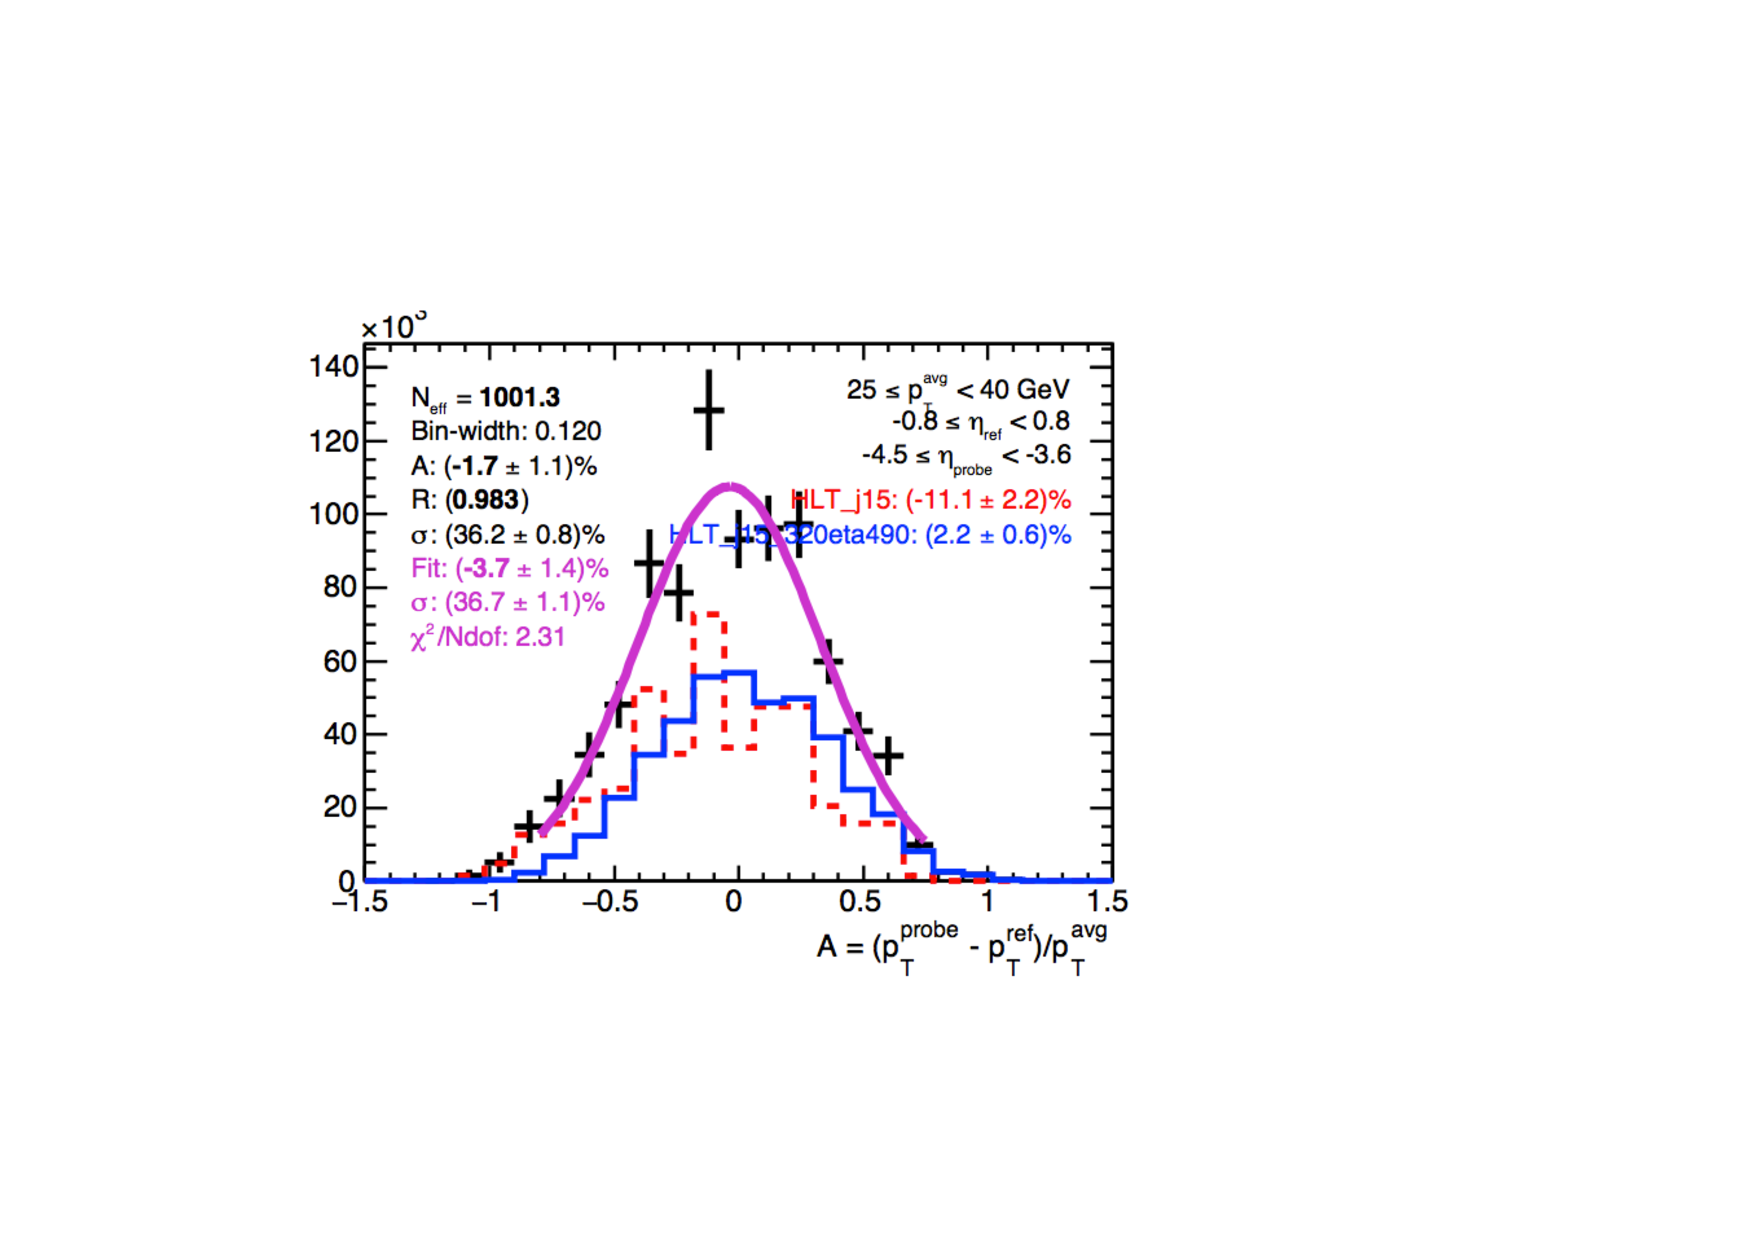
\includegraphics[width=3cm, height=1.75cm]{JER_fit_25to40_Data.pdf}
\center{MC EMTopo}
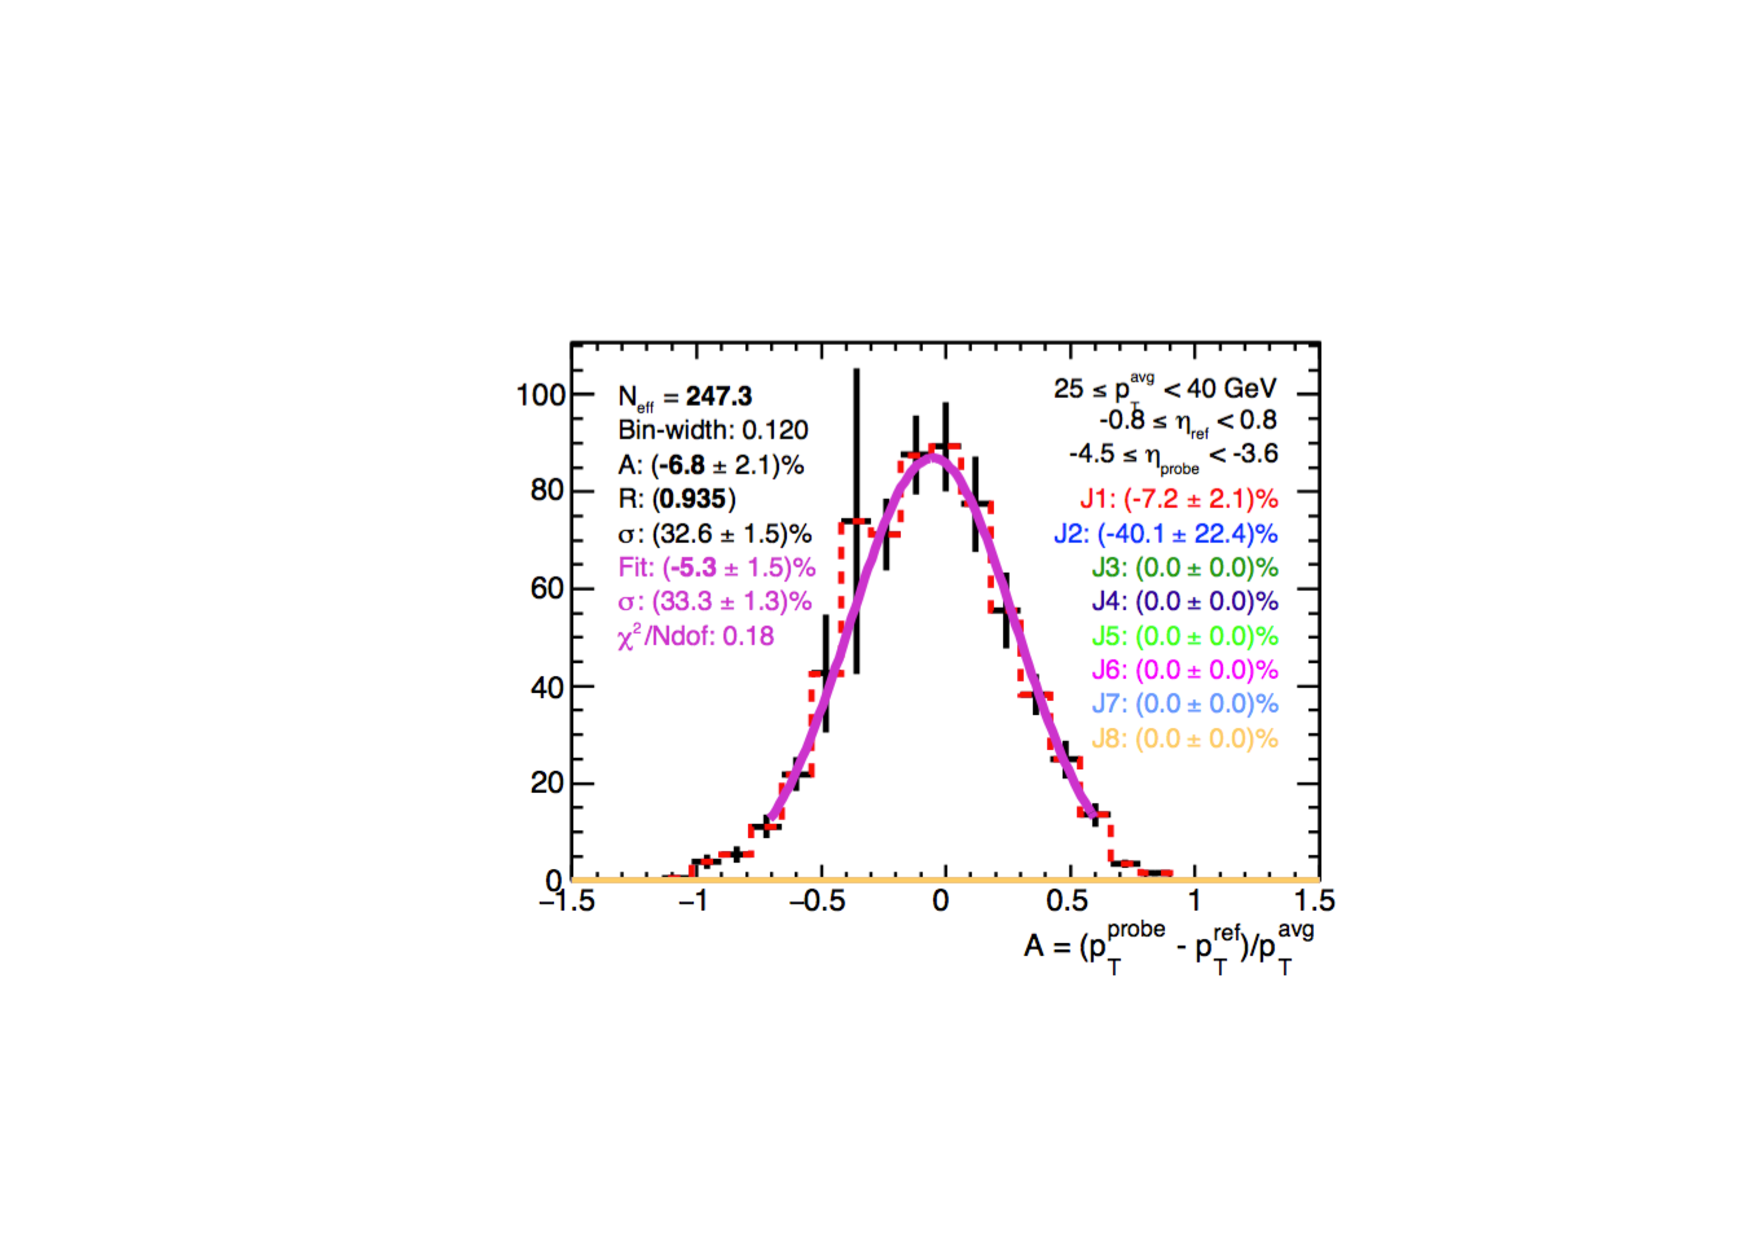
\includegraphics[width=3cm, height=1.75cm]{JER_fit_25to40_EMTopo.pdf}
\center{MC Truth}
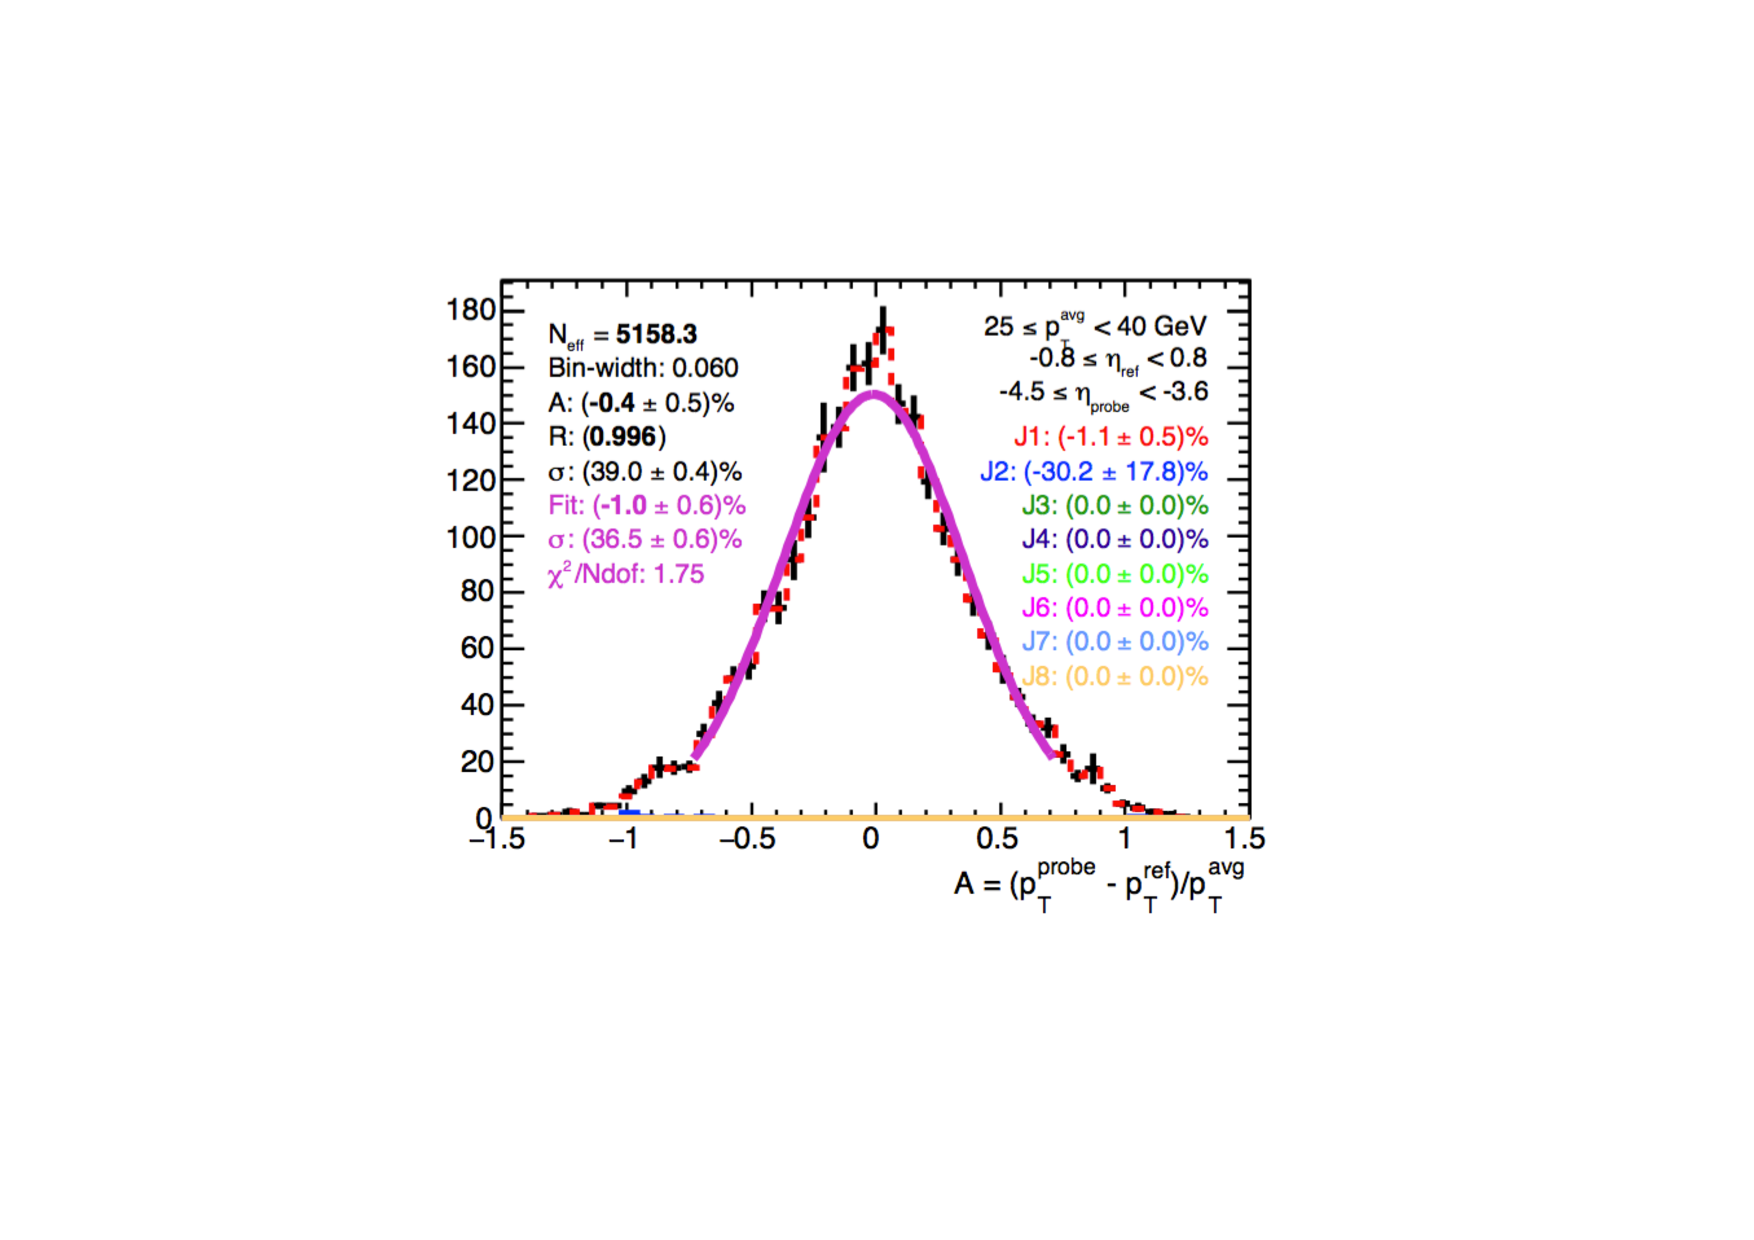
\includegraphics[width=3cm, height=1.75cm]{JER_fit_25to40_Truth.pdf}
\end{column}
\begin{column}{.4\textwidth}
\begin{itemize}
\item The fit doesn't take into account the possibility of a double gaussian.
\item Going to try narrowing this bin range that the fit runs over to see if this affects this plot. 
\end{itemize}
\end{column}
\end{columns}
\end{frame}

\begin{frame}
\frametitle{JER vs Eta}
\begin{columns}
\begin{column}{.3\textwidth}
\includegraphics[width=3.5cm, height=2.5cm]{145pTavg175_MCvsData.pdf}
\newline
\includegraphics[width=3.5cm, height=2.5cm]{175pTavg220_MCvsData.pdf}
\end{column}
\begin{column}{.3\textwidth}
\includegraphics[width=3.5cm, height=2.5cm]{220pTavg270_MCvsData.pdf}
\newline
\includegraphics[width=3.5cm, height=2.5cm]{270pTavg330_MCvsData.pdf}
\end{column}
\begin{column}{.3\textwidth}
\includegraphics[width=3.5cm, height=2.5cm]{400pTavg525_MCvsData.pdf}
\newline
\includegraphics[width=3.5cm, height=2.5cm]{760pTavg1200_MCvsData.pdf}
\end{column}
\end{columns}
\begin{itemize}
\item The other pT ranges are mostly as would be expected. 
\item However, there are a few issues with a lack of statistics in some of the fits that affects two pT ranges: 330 $<$ pTavg $<$ 400 and 525 $<$ pTavg $<$ 760.
\end{itemize}
\end{frame}

\begin{frame}
\frametitle{Problems with the fit}
\begin{columns}
\begin{column}{.3\textwidth}
\includegraphics[width=4.5cm, height=3cm]{330pTavg400_MCvsData.pdf}
\newline
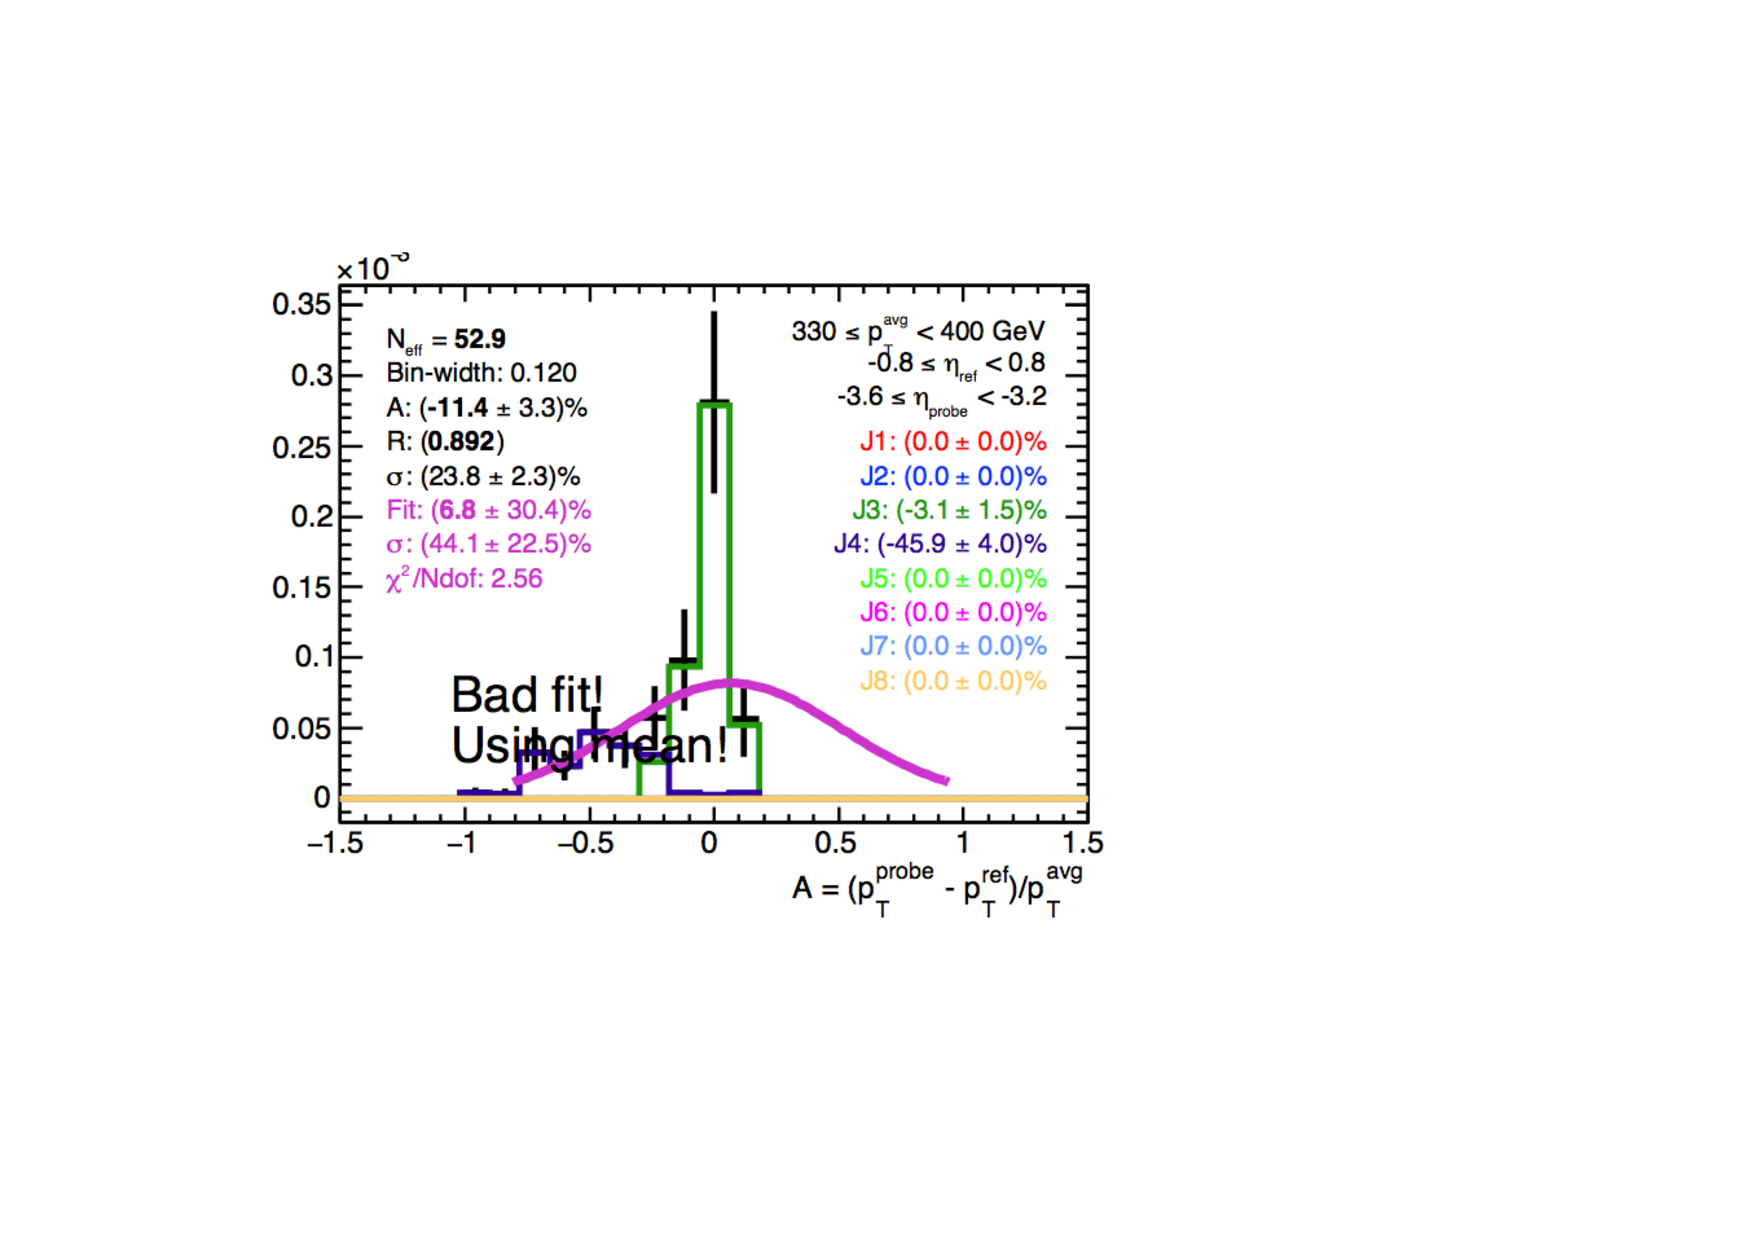
\includegraphics[width=4.5cm, height=3cm]{JER_fit_330to400_Truth.pdf}
\end{column}
\begin{column}{.4\textwidth}
\includegraphics[width=4.5cm, height=3cm]{525pTavg760_MCvsData.pdf}
\newline
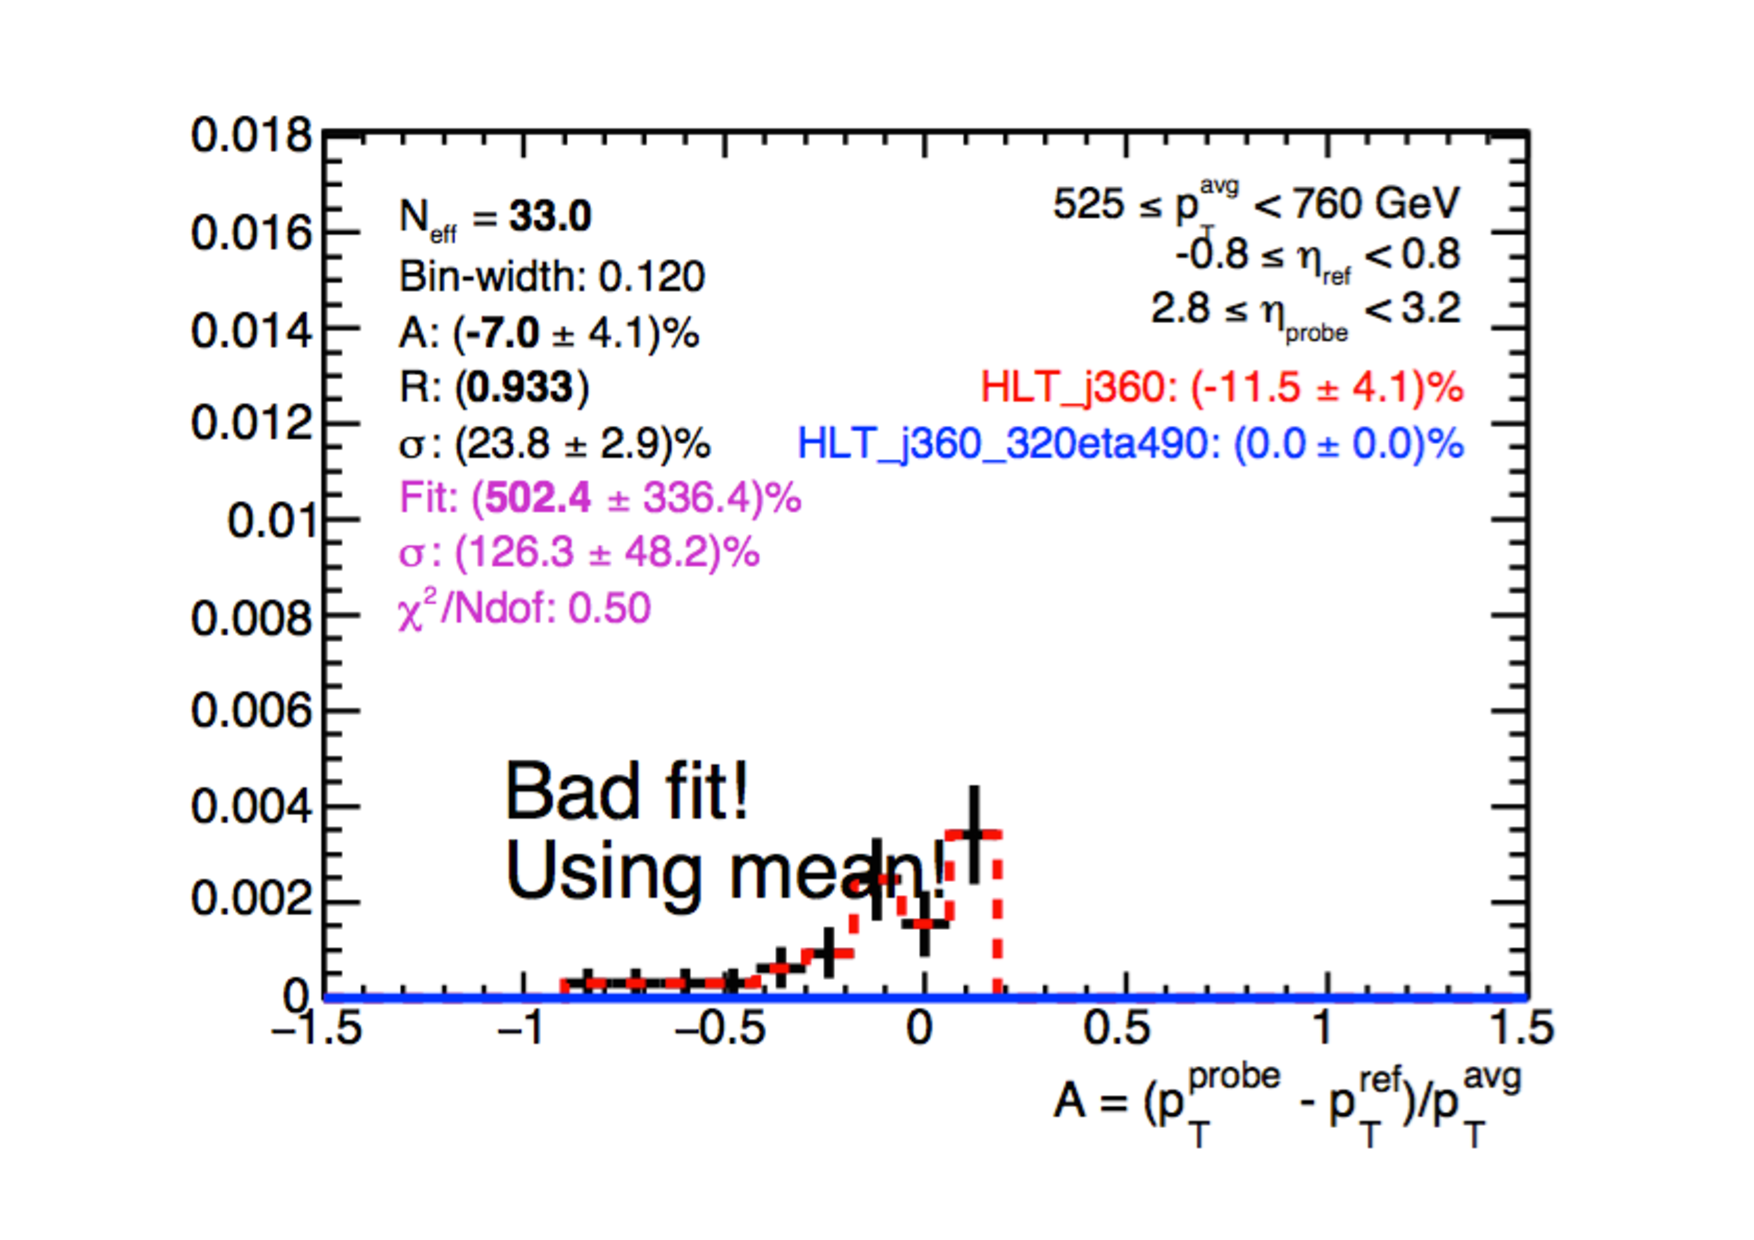
\includegraphics[width=4.5cm, height=3cm]{JER_fit_525to760.pdf}
\end{column}
\end{columns}
\begin{itemize}
\item Both cases have bad fits due to low statistics in these bins. The mean is used - doesn't always work due to weighting problems.
\item Going to look into changing the bin sizes and restricting the rms value when the fit fails.
\end{itemize}
\end{frame}

\begin{frame}
\frametitle{JER vs pT}
\begin{columns}
\begin{column}{.3\textwidth}
\includegraphics[width=4cm, height=3cm]{etaBin4_MCvsData.pdf}
\newline
\includegraphics[width=4cm, height=3cm]{etaBin6_MCvsData.pdf}
\end{column}
\begin{column}{.3\textwidth}
\includegraphics[width=4cm, height=3cm]{etaBin8_MCvsData.pdf}
\newline
\includegraphics[width=4cm, height=3cm]{etaBin10_MCvsData.pdf}
\end{column}
\begin{column}{.3\textwidth}
\includegraphics[width=4cm, height=3cm]{etaBin12_MCvsData.pdf}
\newline
\includegraphics[width=4cm, height=3cm]{etaBin14_MCvsData.pdf}
\end{column}
\end{columns}
\begin{itemize}
\item There is turn-over behaviour in data at low pT causing crossing that isn't understood - and not consistent with MC truth.
\end{itemize}
\end{frame}

\begin{frame}
\frametitle{\small{$\sqrt{(\sigma_{jet})^{2}-(\sigma_{Truth}^{MC})^{2}}$}}
\begin{columns}
\begin{column}{.3\textwidth}
\includegraphics[width=4.5cm, height=3cm]{55pTavg70_Difference.pdf}
\newline
\includegraphics[width=4.5cm, height=3cm]{85pTavg115_Difference.pdf}
\end{column}
\begin{column}{.4\textwidth}
\includegraphics[width=4.5cm, height=3cm]{175pTavg220_Difference.pdf}
\newline
\includegraphics[width=4.5cm, height=3cm]{400pTavg525_Difference.pdf}
\end{column}
\end{columns}
\begin{itemize}
\item Difference plots with Powheg+Pythia8 MC Truth.
\end{itemize}
\end{frame}

\begin{frame}
\frametitle{Next Steps:}
\begin{itemize}
\item Study systematically varied MC subtractions eg. Sherpa
\item Extract a mean resolution from the data and compare with the MC simulated resolution and other systematic studies
\item Study the issues with the fits and bin widths, specifically looking at the lowest and highest bins. Look at merging the last bins/ dropping the bin
\item Repeat with the Bisector method and compare
\item Any suggestions for other studies?
\end{itemize}
\end{frame}



\end{document} 